\documentclass[conference,a4paper]{IEEEtran}
\pdfminorversion=6
\usepackage[utf8]{inputenc}
\usepackage{cite,amsmath,amssymb,graphicx,booktabs,url,microtype,balance}
\begin{document}
\title{Two Distributions, Opposite Verdicts: Feature Provenance in Cross-Dataset Federated Intrusion Detection}
\author{\IEEEauthorblockN{Hoang Tu Trinh and Tien Thanh Cao}
\IEEEauthorblockA{\textit{Faculty of Information Technology}\\
\textit{Ho Chi Minh City University of Foreign Languages -- Information Technology}\\
Ho Chi Minh City, Vietnam\\ Email: tht.csec2005@gmail.com, thanhct@huflit.edu.vn}}
\maketitle
\begin{abstract}
Cross-dataset intrusion-detection results are usually attributed to distribution shift between corpora. We show that for a fixed source model and fixed target traffic, the published verdict can instead be decided by which public CSV distribution of the target dataset the features were taken from. We train logistic-regression FedAvg on InSDN in a five-client, five-seed setting and evaluate it zero-shot on two mirrors built from the same CICIDS2017 traffic. The mirror derived from \texttt{TrafficLabelling}, which retains the original \texttt{Protocol} and \texttt{Source Port} columns, gives ROC-AUC $0.7357$ and MCC $+0.2511$. The mirror derived from \texttt{MachineLearningCVE}, which lacks both columns and therefore infers protocol from TCP flags and substitutes a port sentinel, gives ROC-AUC $0.3441$ and MCC $-0.2698$: a below-random result that would be reported as negative transfer. Masking localizes the mechanism to protocol, whose contribution changes sign across the two mirrors ($-0.1438$ versus $+0.2103$ ROC-AUC), while its marginal Kolmogorov--Smirnov distance is the \emph{smaller} of the two. We then propose a screen that needs no target labels, only source-training statistics and unlabelled target values. It flags the substituted port column on every seed with no false positive among 18 column--mirror pairs, yet no distribution-distance rule separates the reconstructed protocol, whose total-variation distance is again the smaller of the two: some provenance damage is mechanically detectable and some must be reported rather than inferred. Source-domain controls are unaffected: centralized, local-only, IID and non-IID FedAvg reach InSDN F1 $0.9567$, $0.9588$, $0.9580$ and $0.9556$, so FedAvg shows no accuracy advantage. Both mirrors are regenerated from public files by the released script and match published SHA-256 checksums.
\end{abstract}
\begin{IEEEkeywords}Federated learning, intrusion detection, cross-dataset evaluation, feature provenance, reproducibility.\end{IEEEkeywords}

\section{Introduction}
Distributed campus networks combine administrative systems, laboratories, residential networks, and heterogeneous Internet-of-Things endpoints. Federated learning (FL) lets participating sites improve a shared model without centralizing raw records~\cite{fedavg,flsurvey}. Cross-dataset tests are the standard way to check whether such a model generalizes beyond its training corpus, and they routinely report severe degradation~\cite{dhooge,xenids,layeghy,cantone}. That degradation is normally explained by differences in traffic, attack mix, or labeling.

This paper reports a different and largely unexamined cause. Widely used corpora are published in more than one flow-feature distribution, and those distributions do not expose the same columns. CICIDS2017 ships a \texttt{TrafficLabelling} release retaining flow identifiers including \texttt{Protocol} and \texttt{Source Port}, and a \texttt{MachineLearningCVE} release that omits them, so a practitioner harmonizing feature names against the second must reconstruct protocol and substitute a placeholder for the missing port. We show that this choice, not the target traffic, can decide whether the experiment concludes that transfer is usable or below random.

We ask three empirical questions: (RQ1) does FedAvg improve over matched centralized and local controls; (RQ2) how does an explicit non-IID partition affect ranking and fixed-threshold measures; and (RQ3) does the target verdict depend on which public distribution the target features came from, and which feature drives that dependence? Claims are restricted to outputs produced by the accompanying evaluation script.

Our contributions are: (i) matched centralized, local-only, IID, and non-IID controls with paired seed-level reporting; (ii) a controlled two-mirror cross-dataset experiment in which the source model, seeds, preprocessing, and target traffic are held fixed and only the target feature provenance varies, yielding opposite verdicts, with a masking diagnostic that localizes the reversal to a single field whose learned contribution changes sign; and (iii) a label-free provenance screen, validated against that diagnostic, which detects substituted placeholder columns without false positives but provably cannot detect a semantically reconstructed column, from which we derive a concrete per-field reporting requirement. Both mirrors are rebuilt from public files by the released script.

\section{Related Work and Research Gap}
\subsection{Federated intrusion detection and client heterogeneity}
FedAvg established sample-weighted aggregation of local updates~\cite{fedavg}, and security surveys distinguish distributed optimization from formal privacy or attack robustness~\cite{flsurvey}. Because non-IID clients cause objective drift, a family of aggregation methods addresses it directly: FedProx constrains local updates with a proximal term~\cite{fedprox}, SCAFFOLD corrects client drift with control variates~\cite{scaffold}, and FedNova normalizes for unequal local work~\cite{fednova}. FL-IDS work spans linear scanning detectors~\cite{scanfl}, 5G experiments with centralized and local controls~\cite{fiveg}, and deep or distillation-based defenses~\cite{flreview,fedkd}. Dataset-centric FL evaluation reports that in-domain scores approach centralized ones while cross-dataset transfer degrades sharply, and it recommends documenting feature harmonization rather than comparing headline accuracy~\cite{datasetcentric}. We deliberately keep the optimizer at plain FedAvg and the model at logistic regression: RQ1--RQ2 isolate the federation setting, and the aggregation variants above are the natural next step rather than a claim of this paper.

\subsection{Cross-dataset NIDS and feature semantics}
Dataset surveys show that collection environment, labeling, traffic generation, and flow extraction constrain valid comparisons~\cite{ringsurvey}. Inter-dataset studies report large degradation even between related CIC corpora~\cite{dhooge}; XeNIDS formalizes cross-evaluation use cases and warns against assuming interchangeable flow fields~\cite{xenids}. Later work finds asymmetric transfer across four datasets~\cite{layeghy} and near-perfect within-domain yet poor cross-dataset performance~\cite{cantone}. Standardized NetFlow feature sets improve generalization but feature influence stays dataset-dependent~\cite{sarhan}, and domain adaptation exists precisely because feature spaces rarely align~\cite{domainadapt}.

\subsection{Dataset defects, tooling, and release variants}
CICIDS2017 has documented defects rather than merely different statistics. Engelen et al.\ report flow-construction and labeling faults~\cite{troubleshoot}; Lanvin et al.\ find packet misordering, duplication, and an unlabeled port scan, and measure the resulting change in detection performance~\cite{lanvin}; Rosay et al.\ audit the released flows and report duplicated features, miscalculated features, and \emph{wrong protocol detection}, noting that the published CSVs cannot be regenerated from the PCAPs with any available extractor version~\cite{rosay}.

This literature establishes that a corpus can be internally faulty and that two corpora are rarely comparable. The gap we address is narrower and, to our knowledge, unquantified: a \emph{single} corpus is distributed in several feature releases exposing different columns, and the release chosen for the target side can invert the sign of a cross-dataset conclusion while traffic, source model, and protocol are unchanged. We hold everything except target feature provenance fixed, report the mechanism, and ask what an automated check could have caught.

\section{Method}
FedAvg aggregates locally updated parameter vectors $\mathbf{w}^{k}_{t+1}$ in proportion to the local sample count $n_k$~\cite{fedavg}:
\begin{equation}
\mathbf{w}_{t+1}=\sum_{k=1}^{K}\frac{n_k}{\sum_j n_j}\mathbf{w}^{k}_{t+1},\quad K=5.
\end{equation}
Each client runs one local pass of binary logistic regression per round, producing $p(y=1\mid\mathbf{x})=\sigma(\mathbf{w}^{\top}\mathbf{x}+b)$. The model is a transparent tabular baseline, not a deep sequence detector; it is chosen so that the cross-mirror comparison cannot be attributed to architecture.

Server and clients begin from the same neutral zero coefficient/intercept state; no client record is used for initialization. Each client performs one \texttt{partial\_fit} pass over its local records, and returned arrays are averaged with the $n_k$ weights above, so a ``local epoch'' is one complete pass rather than a mini-batch count. Centralized LR uses the same optimizer and 20 complete passes; local-only LR keeps independent client states and averages their test metrics. For each feature, the source-training mean and standard deviation define the z-score and are retained unchanged for the InSDN test partition and both mirrors; non-finite rates and missing values become zero before that fit.

\subsection{Feature-shift diagnostic}
For source feature $j$ with empirical CDF $F_{sj}$ and mirror CDF $F_{tj}$, we record the two-sample Kolmogorov--Smirnov distance
\begin{equation}
D_j=\sup_x\left|F_{sj}(x)-F_{tj}(x)\right|.
\end{equation}
This marginal statistic cannot reveal whether a learned association changes sign. We therefore keep the trained IID global model fixed, replace one standardized feature by zero (the source-training mean) in both test domains, and compute $\Delta A_j=A^{\mathrm{mask}(j)}_t-A^{\mathrm{full}}_t$ for target ROC-AUC. A positive $\Delta A_j$ identifies a feature whose learned contribution harms target ranking; a negative one identifies a feature carrying transferable signal. For a linear score the masked logit is exactly $\mathbf{w}^{\top}\mathbf{x}-w_jx_j$, so the diagnostic is cheap and exact here, and it applies unchanged to nonlinear scores. It does, however, consume target labels, so it audits a finished experiment and cannot protect one in progress.

\subsection{Label-free provenance screen}
We therefore ask what can be established before any target label is available, using only the source-training column $x_j$ and the unlabelled target column $\tilde{x}_j$. The screen raises a flag when either
\begin{equation}
\frac{\mathrm{sd}(\tilde{x}_j)}{\mathrm{sd}(x_j)}<\tau_v
\quad\text{or}\quad
\Pr\!\left[\tilde{x}_j\notin[\min x_j,\max x_j]\right]>\tau_r,
\end{equation}
with $\tau_v=\tau_r=0.01$. The first condition detects a column that has lost essentially all of its variation, the second a column whose values were never observed during training; a placeholder written in place of an absent field triggers both. The thresholds are deliberately one-sided, because a \emph{large} dispersion ratio is ordinary domain shift rather than missing data. For integer-coded fields we also record two candidate rules: the total-variation distance between category proportions, and whether any category holding over 5\% of source mass falls below 1\% of target mass. The label-based $\Delta A_j$ is the ground truth against which all of these are scored.

\section{Experimental Protocol}
\subsection{Source data and the two target mirrors}
We use InSDN~\cite{insdn} for training and within-domain testing. The prepared InSDN file contains 343,889 records (68,424 \texttt{normal}; 275,465 \texttt{anomaly}) and carries true IANA protocol numbers $\{0,6,17\}$. Each seed draws a stratified 30,000-record sample, split into 24,000 train and 6,000 test records, and draws 30,000 records from each mirror.

Both mirrors describe the \emph{same} CICIDS2017 traffic~\cite{cicids}: Monday benign, Friday DDoS, and Friday PortScan. They differ only in the released CSV distribution their columns come from (Table~\ref{tab:mirrors}). The \textsc{tl} mirror comes from \texttt{TrafficLabelling} and keeps the original \texttt{Protocol} and \texttt{Source Port} fields. The \textsc{ml} mirror comes from \texttt{MachineLearningCVE}, where neither column exists, so the script infers protocol as TCP (6) when any TCP flag is positive and 0 otherwise and writes $-1$ for every source port. This is exactly the harmonization a practitioner performs when only that release is at hand, and the script records which branch was taken per input file.

\begin{table}[t]\caption{The two target mirrors. Same traffic and same three labels; only the released CSV distribution differs.}\label{tab:mirrors}\centering\footnotesize
\resizebox{\columnwidth}{!}{\begin{tabular}{lcc}\toprule
& \textsc{tl} mirror & \textsc{ml} mirror\\
& (\texttt{TrafficLabelling}) & (\texttt{MachineLearningCVE})\\\midrule
Protocol field & original column & inferred from TCP flags\\
Protocol values & $\{0,6,17\}$ & $\{0,6\}$\\
Source port field & original column & sentinel $-1$ (all rows)\\
Cleaned flows & 1,037,315 & 880,176\\
Fixed test split & 207,463 & 176,036\\
Sampled benign/attack & 21,705 / 8,295 & 22,577 / 7,423\\
Attack prevalence & 0.2765 & 0.2474\\\bottomrule
\end{tabular}}\end{table}

The nine fields in Table~\ref{tab:map} are the complete input, referenced by name rather than by position. The prepared CSVs also carry a \texttt{flow\_duration} column that is identical to \texttt{duration\_sec} in every row, an instance of the feature duplication reported for these releases~\cite{rosay}; it is excluded so that no coefficient is split across duplicated inputs. Labels are reduced to binary: InSDN \texttt{normal}$\rightarrow0$ and \texttt{anomaly}$\rightarrow1$, giving mean sampled counts of 5,969 benign and 24,031 attack, while in both mirrors \texttt{normal}$\rightarrow0$ and \texttt{ddos}/\texttt{portscan}$\rightarrow1$. Sampling occurs after label conversion and numeric cleanup and is stratified to retain prevalence. No SMOTE output, source string, run identifier, or label field is supplied to the classifier.

\begin{table}[t]\caption{Exact nine-column feature mapping. Names are the canonical column names in the prepared InSDN CSV and in both mirrors. Ports span 0--65,535 except for the \textsc{ml} sentinel $-1$.}\label{tab:map}\centering\footnotesize
\scriptsize\setlength{\tabcolsep}{3pt}\begin{tabular}{p{.20\columnwidth}p{.38\columnwidth}p{.29\columnwidth}}
\toprule Feature & CSV column & Transformation\\\midrule
Protocol & \texttt{ip\_proto} & z-score; one-hot in ablation\\
Source port & \texttt{tp\_src} & z-score; dropped by ports ablation\\
Destination port & \texttt{tp\_dst} & z-score; dropped by ports ablation\\
Packet count & \texttt{packet\_count} & z-score\\
Byte count & \texttt{byte\_count} & z-score\\
Duration & \texttt{duration\_sec} & z-score (seconds)\\
Packet rate & \texttt{packet\_count\_per\_sec} & Inf/NaN $\rightarrow0$; z-score\\
Byte rate & \texttt{byte\_count\_per\_sec} & Inf/NaN $\rightarrow0$; z-score\\
Mean packet size & \texttt{packet\_size\_avg} & z-score (bytes)\\\bottomrule
\end{tabular}\end{table}

\texttt{StandardScaler} is fit once on the InSDN training features and applied unchanged to the InSDN test partition and both mirrors; no target-domain fit, fine-tuning, or threshold selection is performed.

\subsection{Partitions and measures}
For IID FL, shuffled training records are divided equally among five clients. For non-IID FL, each class is allocated using a Dirichlet distribution with $\alpha=0.5$. Both configurations run 20 rounds fixed \emph{a priori}; no early stopping, model selection, or tuning uses the test set. We report precision, recall, F1, ROC-AUC, PR-AUC, balanced accuracy, MCC, and confusion matrices. The random PR baseline equals the attack prevalence: 0.801 in InSDN and the mirror values in Table~\ref{tab:mirrors}.

Predicted attack labels use the fixed probability threshold 0.5, ROC-AUC and PR-AUC use continuous scores, and F1 uses the corresponding hard labels. Balanced accuracy prevents the majority attack class from dominating the summary, while MCC incorporates all four confusion cells and its sign makes a below-random operating point immediately visible. The saved CSV records every metric for each seed, setting, and target domain.

IID partitioning gives every client 4,800 records and retains class proportions (benign counts 925--1,000 at seed 11), whereas the Dirichlet split intentionally produces severe skew: at the same seed, client sizes range from 1,669 to 11,950 records and the benign share from 0.5\% (23 of 4,842) to 38\% (758 of 1,986). The same seeded procedure is rerun for each seed and every partition is recorded in the artifact. Centralized LR uses the identical 24,000 training records; local-only LR trains five independently initialized client models and reports their unweighted metric mean.

\begin{table}[t]\caption{Implementation and protocol.}\label{tab:hyper}\centering\resizebox{\columnwidth}{!}{\begin{tabular}{ll}\toprule
Item & Setting\\\midrule
Classifier & scikit-learn SGDClassifier, \texttt{log\_loss}\\
Optimizer & constant SGD, $\eta=0.01$, L2 $\alpha=10^{-4}$\\
Initialization & shared zero coefficients/intercept; no client data\\
Class weighting / threshold & none / 0.5 fixed\\
Clients, rounds, local work & 5, 20, one full local pass per round\\
Seeds & 11, 23, 42, 77, 101\\
NaN/Inf & replace Inf by NaN, then 0 before scaling\\
Environment & Python 3.11; NumPy 2.2.6; pandas 2.3.1; scikit-learn 1.7.2\\\bottomrule\end{tabular}}\end{table}

\section{Results}
\subsection{Source-domain controls}
Table~\ref{tab:results} contains mean$\pm$standard deviation over five seeded repeated holdouts/partitions. All four configurations reach F1 around $0.956$--$0.959$: FedAvg IID lies between the centralized and local-only controls, and the gap to centralized is smaller than the seed-to-seed standard deviations. Local-only attains the highest mean F1, but this is not evidence of superiority because it is an unweighted mean over five models scored on the common test set. Non-IID allocation preserves ROC-AUC while reducing balanced accuracy and MCC, consistent with an operating-point effect under client class skew rather than a uniformly worse ranking of examples.
\begin{table}[t]
\caption{Source-domain (InSDN) five-seed results; mean$\pm$std.}\label{tab:results}\centering\scriptsize\setlength{\tabcolsep}{2.5pt}
\begin{tabular}{lrrrr}\toprule
Setting&F1&ROC-AUC&Bal. acc.&MCC\\\midrule
Central&.9567$\pm$.0033&.9320$\pm$.0038&.8285$\pm$.0149&.7624$\pm$.0199\\
Local-only&.9588$\pm$.0027&.9288$\pm$.0030&.8367$\pm$.0120&.7751$\pm$.0162\\
FedAvg IID&.9580$\pm$.0023&.9324$\pm$.0039&.8355$\pm$.0091&.7709$\pm$.0140\\
FedAvg non-IID&.9556$\pm$.0038&.9336$\pm$.0064&.8136$\pm$.0166&.7562$\pm$.0228\\\bottomrule
\end{tabular}\end{table}
\begin{table}[t]
\caption{Seed-level federated results on the common InSDN test protocol, before mean$\pm$std aggregation. ROC-AUC and balanced accuracy per seed are in \texttt{five\_seed\_metrics.csv}.}\label{tab:seed}
\centering\scriptsize
\begin{tabular}{crr|rr}
\toprule
&\multicolumn{2}{c|}{FedAvg IID}&\multicolumn{2}{c}{Dirichlet $\alpha=.5$}\\
Seed&F1&MCC&F1&MCC\\\midrule
11&.9604&.7848&.9570&.7653\\
23&.9575&.7678&.9543&.7489\\
42&.9557&.7569&.9543&.7485\\
77&.9560&.7586&.9510&.7284\\
101&.9606&.7862&.9611&.7897\\\bottomrule
\end{tabular}
\end{table}
\begin{figure}[t]\centering
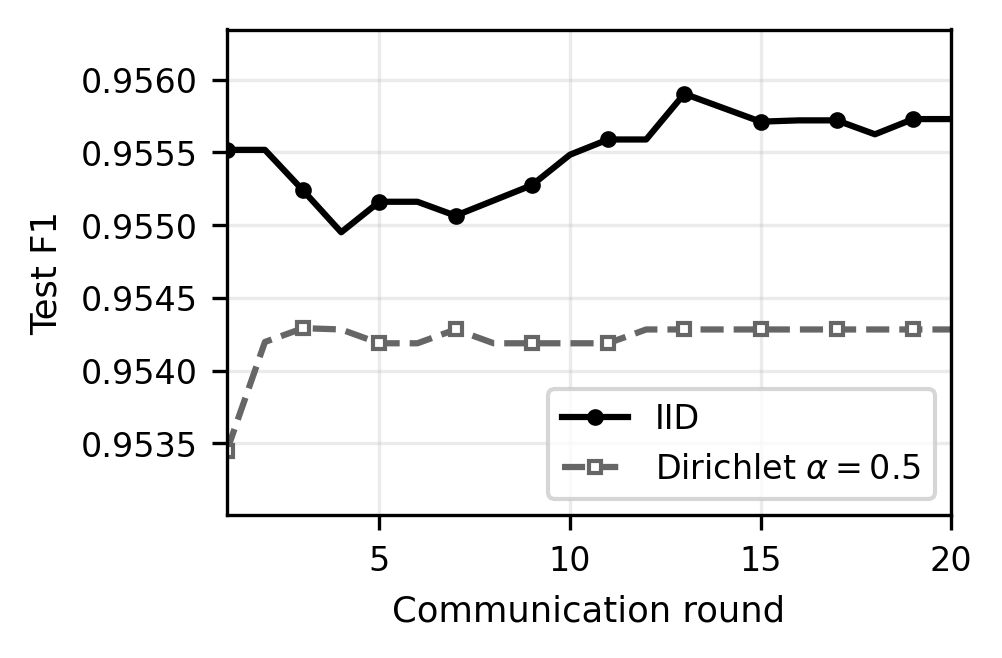
\includegraphics[width=\columnwidth]{paper/figures/verified/fedavg_convergence.png}
\caption{Seed-42 descriptive test F1 over 20 fixed communication rounds. The y-axis is zoomed to expose the small difference; solid/circle denotes IID and dashed/square denotes non-IID.}\label{fig:convergence}\end{figure}
Figure~\ref{fig:convergence} is rendered from the saved seed-42 round-wise CSV. It is descriptive rather than a model-selection curve: round 20 was fixed before evaluation, and no displayed point controls stopping or tuning.

For seed 11, the IID FedAvg confusion matrix contains TN=833, FP=361, FN=33, and TP=4,773, so the class imbalance explains why F1 and PR-AUC alone are insufficient and why Table~\ref{tab:results} includes MCC. Table~\ref{tab:seed} makes the aggregation transparent: IID FedAvg F1 ranges from 0.9557 to 0.9606, and the non-IID range is wider (0.9510--0.9611), as expected when both sampled records and client allocations change.

\subsection{The two mirrors give opposite verdicts}
The same five IID FedAvg models are now scored on both mirrors without any refitting. Table~\ref{tab:cross} shows that the conclusion depends on provenance, not on traffic. On the \textsc{tl} mirror, transfer is clearly degraded relative to the source domain ($0.9324\rightarrow0.7357$ ROC-AUC) but remains informative, with positive MCC and PR-AUC $0.4520$ against a $0.2765$ prevalence baseline. On the \textsc{ml} mirror the same models fall below chance on every measure, with ROC-AUC $0.3441$ and MCC $-0.2698$. Reported alone, the second row is a negative-transfer result; reported alone, the first row is an ordinary domain-shift result. The seed-to-seed standard deviations are two orders of magnitude smaller than the gap, so this is not sampling noise.
\begin{table}[t]
\caption{Zero-shot cross-dataset results by mirror, five seeds. Identical source models, identical target traffic.}\label{tab:cross}\centering\scriptsize\setlength{\tabcolsep}{2.5pt}
\resizebox{\columnwidth}{!}{\begin{tabular}{lrrrrr}\toprule
Mirror&F1&ROC-AUC&PR-AUC&Bal. acc.&MCC\\\midrule
\textsc{tl} (original fields)&.5012$\pm$.0037&.7357$\pm$.0070&.4520$\pm$.0154&.6403$\pm$.0037&.2511$\pm$.0065\\
\textsc{ml} (inferred fields)&.2914$\pm$.0018&.3441$\pm$.0040&.1848$\pm$.0010&.3766$\pm$.0023&-.2698$\pm$.0067\\\bottomrule
\end{tabular}}\end{table}

\subsection{Localizing the reversal}
Table~\ref{tab:audit} perturbs the fixed model one feature at a time. Protocol is the only field whose masking effect changes sign between the mirrors. On \textsc{tl} it carries the largest transferable contribution: masking it costs $0.1438$ ROC-AUC, the biggest loss of any feature. On \textsc{ml} the flag-derived surrogate does the opposite, and removing it \emph{gains} $0.2103$. Marginal shift magnitude does not identify this: the KS distance for protocol is $0.3532$ on \textsc{tl} and only $0.0992$ on \textsc{ml}, so the harmful encoding is the one that looks better aligned. Source port illustrates the converse failure of KS as a screen: on \textsc{ml} its distance is maximal because every value is the sentinel, yet masking it changes nothing at all.
\begin{table}[t]\caption{Model-preserving feature audit; five-seed means. $\Delta$AUC is masked minus full mirror ROC-AUC. Source F1 is shared because the source model is identical.}\label{tab:audit}\centering\footnotesize\setlength{\tabcolsep}{4pt}
\begin{tabular}{lrrrrr}\toprule
&&\multicolumn{2}{c}{\textsc{tl} mirror}&\multicolumn{2}{c}{\textsc{ml} mirror}\\
\cmidrule(lr){3-4}\cmidrule(lr){5-6}
Masked feature&Src. F1&KS&$\Delta$AUC&KS&$\Delta$AUC\\\midrule
Protocol&.9070&.3532&-.1438&.0992&+.2103\\
Destination port&.9611&.3533&-.0605&.3535&-.0583\\
Mean packet size&.9500&.5642&+.0547&.5571&+.0639\\
Source port&.9563&.4287&+.0165&1.0000&.0000\\\bottomrule
\end{tabular}\end{table}

Retraining confirms the mechanism rather than inferring it from perturbation alone. Table~\ref{tab:ablation} removes fields before training. Dropping protocol costs source F1 ($0.9580\rightarrow0.9118$) and collapses \emph{both} mirrors to approximately chance ($0.4953$ and $0.4668$): once protocol is gone, the two provenances agree, because the field they disagree about is no longer used. One-hot encoding protocol is the best \textsc{tl} configuration ($0.7472$) yet barely moves \textsc{ml} ($0.3506$), so a representation change cannot repair a field whose values were reconstructed. Removing both ports lowers \textsc{tl} ROC-AUC from $0.7357$ to $0.7062$ while leaving source F1 unchanged, indicating genuine but secondary port signal that the \textsc{ml} release cannot express at all.
\begin{table}[t]\caption{Retraining ablations, five seeds. Source columns are InSDN; mirror columns are zero-shot ROC-AUC.}\label{tab:ablation}\centering\scriptsize\setlength{\tabcolsep}{3pt}
\begin{tabular}{lrrrr}\toprule
Features&Src. F1&Src. ROC-AUC&\textsc{tl} AUC&\textsc{ml} AUC\\\midrule
All nine&.9580$\pm$.0023&.9324$\pm$.0039&.7357$\pm$.0070&.3441$\pm$.0040\\
Without ports&.9583$\pm$.0030&.9267$\pm$.0065&.7062$\pm$.0083&.2857$\pm$.0032\\
Without protocol&.9118$\pm$.0042&.8915$\pm$.0067&.4953$\pm$.0112&.4668$\pm$.0082\\
One-hot protocol&.9582$\pm$.0023&.9311$\pm$.0036&.7472$\pm$.0074&.3506$\pm$.0047\\\bottomrule
\end{tabular}\end{table}

\subsection{What a label-free screen can and cannot catch}\label{sec:screen}
Table~\ref{tab:screen} applies the screen of Section~III-B, which sees no target label. Across all 18 column--mirror pairs it raises exactly one flag, on the \textsc{ml} source port, on all five seeds: that column retains none of its variation (ratio $0.0000$) and every target row lies outside the source-training range. There is no false positive, and the margins are wide because no unflagged column falls below ratio $0.352$ or exceeds out-of-range $0.0028$. The same table justifies the one-sided thresholds: the byte-rate column is 31 to 48 times more dispersed in the target, yet its $\Delta$AUC is $0.0000$, so a large dispersion change is not by itself a defect.

The screen cannot, however, catch the field that actually reverses the verdict. The \textsc{ml} protocol column keeps a plausible dispersion ratio ($0.5606$) and never leaves the source range, so both conditions stay silent, and neither candidate categorical rule repairs this. Total-variation distance repeats the failure already seen for KS, scoring the harmful encoding as the \emph{closer} one ($0.1611$ against $0.3532$). The mass-collapse rule fires on \emph{both} mirrors, since \textsc{ml} drops IANA protocol 17 entirely while \textsc{tl} reduces protocol 0 from $35\%$ of source mass to $0.04\%$; a rule that fires on the benign mirror as readily as on the damaged one cannot discriminate, so we report the negative result rather than tune a threshold until the cases separate.
\begin{table}[t]\caption{Label-free screen, five-seed means. Ratio is target over source-training standard deviation; OOR is the fraction of target rows outside the source-training range. A flag requires ratio $<0.01$ or OOR $>0.01$; the only flagged cell pair is shown in bold.}\label{tab:screen}\centering\footnotesize\setlength{\tabcolsep}{4pt}
\begin{tabular}{lrrrr}\toprule
&\multicolumn{2}{c}{\textsc{tl} mirror}&\multicolumn{2}{c}{\textsc{ml} mirror}\\
\cmidrule(lr){2-3}\cmidrule(lr){4-5}
Column&Ratio&OOR&Ratio&OOR\\\midrule
Protocol&1.0401&.0000&0.5606&.0000\\
Source port&0.9481&.0028&\textbf{0.0000}&\textbf{1.0000}\\
Destination port&1.1984&.0005&1.2650&.0006\\
Byte rate&30.6377&.0023&47.6245&.0028\\\bottomrule
\end{tabular}\end{table}

The consequence is a division of labour. Substituted placeholders are mechanically detectable, so an artifact should be rejected when the screen fires. A field reconstructed from a different signal leaves no statistical trace in the target column and can only be known from provenance metadata recorded at preparation time, which is why our script records per input file whether each such field was read or reconstructed.

\section{Discussion}
\subsection{What the controls establish}
The controls share the feature set, train/test records, optimizer family, class weight, and decision threshold, so their close source-domain scores establish only that this lightweight linear baseline is adequate for the sampled InSDN binary task. They do not establish that federated learning improves accuracy, and the appropriate conclusion is feasibility and reproducibility of the protocol. The non-IID experiment makes a narrower point: under the client skew described in Section~IV-B, mean F1 decreases only slightly while balanced accuracy and MCC decrease more visibly, so reporting all three prevents high attack prevalence from hiding an unfavorable tradeoff. More severe non-IID settings, drift-corrected aggregation~\cite{fedprox,scaffold,fednova}, client dropout, Byzantine clients, privacy accounting, and communication cost are outside this experiment.

\subsection{Why provenance, not traffic, is the operative variable}
Because the two mirrors describe the same days of the same capture and are scored by the same models under the same source-fitted scaler and threshold, the difference in Table~\ref{tab:cross} cannot be attributed to attack mix, labeling, or collection environment. It is produced by the reconstruction the \textsc{ml} release forces: protocol becomes a TCP-flag indicator that omits UDP entirely, and source port becomes a constant. This is why the effect is a reversal rather than a loss. The model applies a coefficient to a field whose target values now encode something else, so its contribution is not merely uninformative but anti-correlated, which drives MCC below zero. Rosay et al.\ independently report wrong protocol detection in these releases~\cite{rosay}; our result quantifies what such a field does to a verdict.

Section~\ref{sec:screen} turns this into an actionable rule with a stated limit. Automated validation is sufficient for placeholder substitution and should be run, but it is provably insufficient for semantic reconstruction, so a cross-dataset NIDS result must state which release of each corpus supplied each feature and which fields were reconstructed rather than read. Absent that record, a below-random result cannot be distinguished from an artifact of harmonization, and neither can a favorable one. Distance statistics are not a substitute: on both KS and total variation, the more harmful of our two protocol encodings is the one that looks closer to the source.

The external evaluation fixes every source-fitted quantity, including scaling and the 0.5 threshold, which is stricter than re-fitting either on target labels. The residual \textsc{tl} degradation still admits several causes, including attack mix, label reduction, and the limited expressiveness of nine aggregate features; this design does not attribute it to any one of them.

\section{Threats to Validity and Reproducibility}
The experiment evaluates tabular flows, not ordered packet traces, and is not an SDN deployment. Five repeated holdouts share a finite source corpus and are not independent sites. The two-mirror contrast covers one source corpus, one target corpus, one model family, and three capture files; whether the reversal generalizes to other release pairs is open, and the \textsc{ml} reconstruction rule is one of several possible ones. The screen's thresholds were fixed at $0.01$ rather than tuned, and its guarantee is one-directional: a flag is strong evidence of substitution, but silence is not evidence of sound provenance. Binary reduction and unequal attack mixes limit external validity. The artifact preserves construction code, per-file field provenance, checksums, seeds, partitions, metrics, histories, and the figure.

\balance
\section{Artifact Availability}
The preparation script converts named public source files, records which branch supplied each reconstructed field, and publishes SHA-256 checksums for the InSDN file and both mirrors, either of which can be rebuilt independently. The evaluation script regenerates the five-seed outputs, the two-mirror audit, the screen, and the figure under the pinned Python 3.11 environment, and a companion script re-reads this paper and fails if any reported value disagrees with the saved outputs. The artifact is at \url{https://github.com/thtcsec/rivf2026-federated-edge}; third-party datasets are not redistributed.

\section{Conclusion}
Matched controls show no FedAvg accuracy advantage on sampled InSDN, while non-IID skew primarily harms fixed-threshold measures. Holding source model, seeds, preprocessing, and target traffic fixed, the released feature distribution chosen for the target side decides the cross-dataset verdict: ROC-AUC $0.7357$ with MCC $+0.2511$ from the original fields, against $0.3441$ with MCC $-0.2698$ when protocol is inferred and ports are unavailable. Masking and retraining localize the reversal to protocol and show that the smaller marginal shift is the more harmful encoding. A screen that uses no target labels then flags the substituted port column with no false positive among 18 column--mirror pairs, but cannot flag the reconstructed protocol, and no distance-based rule we tested separates the two encodings. Automated checks should therefore be run for placeholder substitution, while semantic reconstruction has to be declared: cross-dataset NIDS evaluations should report feature provenance per field. Future work should test whether the reversal persists across other corpora, release pairs, and model families.
\section*{Acknowledgment}
The authors thank the Faculty of Information Technology at Ho Chi Minh City University of Foreign Languages -- Information Technology for academic support.
\textbf{Generative AI Disclosure}: OpenAI Codex and Cursor assisted language drafting and script refactoring; they generated no experimental data or numerical result. The authors executed the code, obtained the public source files, verified every source and output, and take responsibility for all text, code, citations, and claims.
\begin{thebibliography}{00}
\bibitem{fedavg} H. B. McMahan, E. Moore, D. Ramage, S. Hampson, and B. A. y Arcas, ``Communication-Efficient Learning of Deep Networks from Decentralized Data,'' in \textit{Proc. AISTATS}, 2017, pp. 1273--1282.
\bibitem{flsurvey} V. Mothukuri \textit{et al.}, ``A Survey on Security and Privacy of Federated Learning,'' \textit{Future Generation Computer Systems}, vol. 115, pp. 619--640, 2021.
\bibitem{dhooge} L. D'hooge, T. Wauters, B. Volckaert, and F. De Turck, ``Inter-Dataset Generalization Strength of Supervised Machine Learning Methods for Intrusion Detection,'' \textit{J. Information Security and Applications}, vol. 54, Art. 102564, 2020, doi: 10.1016/j.jisa.2020.102564.
\bibitem{xenids} G. Apruzzese, L. Pajola, and M. Conti, ``The Cross-Evaluation of Machine Learning-Based Network Intrusion Detection Systems,'' \textit{IEEE Trans. Network and Service Management}, vol. 19, no. 4, pp. 5152--5169, 2022, doi: 10.1109/TNSM.2022.3157344.
\bibitem{layeghy} S. Layeghy and M. Portmann, ``Explainable Cross-Domain Evaluation of ML-Based Network Intrusion Detection Systems,'' \textit{Computers and Electrical Engineering}, vol. 108, Art. 108692, 2023, doi: 10.1016/j.compeleceng.2023.108692.
\bibitem{cantone} M. Cantone, C. Marrocco, and A. Bria, ``Machine Learning in Network Intrusion Detection: A Cross-Dataset Generalization Study,'' \textit{IEEE Access}, vol. 12, pp. 144489--144508, 2024, doi: 10.1109/ACCESS.2024.3472907.
\bibitem{fedprox} T. Li \textit{et al.}, ``Federated Optimization in Heterogeneous Networks,'' in \textit{Proc. Machine Learning and Systems (MLSys)}, vol. 2, 2020, pp. 429--450.
\bibitem{scaffold} S. P. Karimireddy \textit{et al.}, ``SCAFFOLD: Stochastic Controlled Averaging for Federated Learning,'' in \textit{Proc. ICML}, PMLR vol. 119, 2020, pp. 5132--5143.
\bibitem{fednova} J. Wang, Q. Liu, H. Liang, G. Joshi, and H. V. Poor, ``Tackling the Objective Inconsistency Problem in Heterogeneous Federated Optimization,'' in \textit{Advances in Neural Information Processing Systems (NeurIPS)}, 2020.
\bibitem{scanfl} R. Doriguzzi-Corin, S. Cretti, and D. Siracusa, ``Improving Detection of Scanning Attacks on Heterogeneous Networks with Federated Learning,'' \textit{ACM SIGMETRICS Performance Evaluation Review}, vol. 49, no. 4, 2022, doi: 10.1145/3543146.3543172.
\bibitem{fiveg} T. E. T. Djaidja, B. Brik, A. Boualouache, S. M. Senouci, and Y. Ghamri-Doudane, ``Federated Learning for 5G and Beyond, a Blessing and a Curse--An Experimental Study on Intrusion Detection Systems,'' \textit{Computers \& Security}, vol. 139, Art. 103707, 2024, doi: 10.1016/j.cose.2024.103707.
\bibitem{flreview} A. Belenguer, J. A. Pascual, and J. Navaridas, ``A Review of Federated Learning Applications in Intrusion Detection Systems,'' \textit{Computer Networks}, vol. 258, Art. 111023, 2025, doi: 10.1016/j.comnet.2024.111023.
\bibitem{fedkd} N. H. Quyen, P. T. Duy, N. T. Nguyen, N. H. Khoa, and V.-H. Pham, ``FedKD-IDS: A Robust Intrusion Detection System Using Knowledge Distillation-Based Semi-Supervised Federated Learning and Anti-Poisoning Attack Mechanism,'' \textit{Information Fusion}, vol. 117, Art. 102807, 2025, doi: 10.1016/j.inffus.2024.102807.
\bibitem{datasetcentric} M. A. Bilal \textit{et al.}, ``Dataset-Centric Evaluation of Federated Intrusion Detection Models in IoT Networks,'' \textit{Scientific Reports}, vol. 16, Art. 2683, 2026, doi: 10.1038/s41598-025-32567-w.
\bibitem{ringsurvey} M. Ring, S. Wunderlich, D. Scheuring, D. Landes, and A. Hotho, ``A Survey of Network-Based Intrusion Detection Data Sets,'' \textit{Computers \& Security}, vol. 86, pp. 147--167, 2019, doi: 10.1016/j.cose.2019.06.005.
\bibitem{sarhan} M. Sarhan, S. Layeghy, and M. Portmann, ``Evaluating Standard Feature Sets Towards Increased Generalisability and Explainability of ML-Based Network Intrusion Detection,'' \textit{Big Data Research}, vol. 30, Art. 100359, 2022, doi: 10.1016/j.bdr.2022.100359.
\bibitem{domainadapt} A. Singla, E. Bertino, and D. Verma, ``Preparing Network Intrusion Detection Deep Learning Models with Minimal Data Using Adversarial Domain Adaptation,'' in \textit{Proc. 15th ACM Asia Conf. Computer and Communications Security (ASIA CCS)}, 2020, pp. 127--140.
\bibitem{troubleshoot} G. Engelen, V. Rimmer, and W. Joosen, ``Troubleshooting an Intrusion Detection Dataset: The CICIDS2017 Case Study,'' in \textit{Proc. IEEE Security and Privacy Workshops}, 2021, pp. 7--12, doi: 10.1109/SPW53761.2021.00009.
\bibitem{lanvin} M. Lanvin \textit{et al.}, ``Errors in the CICIDS2017 Dataset and the Significant Differences in Detection Performances It Makes,'' in \textit{Risks and Security of Internet and Systems (CRiSIS)}, LNCS vol. 13857, Springer, 2022, pp. 18--33, doi: 10.1007/978-3-031-31108-6\_2.
\bibitem{rosay} A. Rosay, E. Cheval, F. Carlier, and P. Leroux, ``Network Intrusion Detection: A Comprehensive Analysis of CIC-IDS2017,'' in \textit{Proc. 8th Int. Conf. Information Systems Security and Privacy (ICISSP)}, 2022, pp. 25--36, doi: 10.5220/0010774000003120.
\bibitem{insdn} M. S. Elsayed, N.-A. Le-Khac, and A. D. Jurcut, ``InSDN: A Novel SDN Intrusion Dataset,'' \textit{IEEE Access}, vol. 8, pp. 165263--165284, 2020, doi: 10.1109/ACCESS.2020.3022633.
\bibitem{cicids} I. Sharafaldin, A. H. Lashkari, and A. A. Ghorbani, ``Toward Generating a New Intrusion Detection Dataset and Intrusion Traffic Characterization,'' in \textit{Proc. ICISSP}, 2018, pp. 108--116.
\end{thebibliography}
\end{document}
